\chapter{Giới thiệu đề tài}
\section{Đặt vấn đề}
\quad Ngành nông nghiệp đóng vai trò quan trọng trong nền kinh tế và cung cấp nguồn thực phẩm thiết yếu cho xã hội. Tuy nhiên, việc mua bán nông sản và dịch vụ nông nghiệp vẫn phụ thuộc chủ yếu vào các phương pháp truyền thống như sử dụng đại lý, thị trường truyền thống hoặc giao dịch trực tiếp giữa các bên liên quan. Các phương pháp này có thể gặp phải nhiều hạn chế, các nhà sản xuất và doanh nghiệp trong ngành nông nghiệp thường gặp khó khăn trong việc tiếp cận thị trường, quảng bá sản phẩm và tìm kiếm khách hàng. Đồng thời, người tiêu dùng cũng gặp rào cản khi muốn tìm kiếm và mua các sản phẩm nông nghiệp chất lượng cao từ các nhà sản xuất đáng tin cậy.

Do đó, cần có một giải pháp số hóa để tạo ra một môi trường kết nối hiệu quả giữa nhà sản xuất, doanh nghiệp và người tiêu dùng trong ngành nông nghiệp. Vì vậy nhu cầu phát triển một nền tảng thương mại điện tử chuyên về nông sản và dịch vụ nông nghiệp là hoàn toàn hợp lý. 

Dự án của chúng tôi hướng tới việc cung cấp một nền tảng cho phép các nhà sản xuất và doanh nghiệp đăng ký và quảng bá sản phẩm của họ, cung cấp thông tin chi tiết về nguồn gốc, chất lượng và phương pháp sản xuất . Đồng thời, người tiêu dùng sẽ có thể dễ dàng tìm kiếm, so sánh và mua các sản phẩm nông nghiệp trực tuyến từ các nhà sản xuất và doanh nghiệp uy tín.

\section{Mục tiêu dự án}
\quad Mục tiêu của dự án xây dựng sàn thương mại điện tử nông sản là tận dụng sức mạnh của công nghệ và nền tảng kỹ thuật số để biến đổi ngành nông nghiệp tại Việt Nam. Dự án nhằm xây dựng một thị trường trực tuyến mạnh mẽ và hiệu quả để kết nối cũng như phục vụ một loạt người dùng đa dạng, từ các doanh nghiệp nông nghiệp quy mô lớn, đến các cửa hàng nông sản nhỏ lẻ, những người sản xuất nông nghiệp và người tiêu dùng sản phẩm.

Một trong những mục tiêu chính của dự án là tạo cơ hội cho nông dân bằng cách cung cấp cho họ quyền tiếp cận trực tiếp đến một tệp khách hàng tiềm năng lớn hơn. Thông qua nền tảng Thương mại điện tử Nông sản, nông dân có thể giới thiệu sản phẩm của mình đến một đối tượng khách hàng rộng hơn, không cần phải thông qua các bên trung gian truyền thống và nhận được giá trị thích đáng hơn cho sản phẩm nông sản của mình. Mối kết nối trực tiếp này không chỉ tăng hiệu quả kinh doanh cho nông dân mà còn giúp họ xây dựng mối quan hệ mạnh mẽ với khách hàng của mình.

Bằng việc xây dựng một sàn thương mại điện tử nông sản, dự án nhằm tối ưu hoá quy trình mua bán sản phẩm nông nghiệp. Nền tảng thương mại điện tử tạo điều kiện giao dịch minh bạch, loại bỏ các bên trung gian không cần thiết, giảm chi phí giao dịch và nâng cao hiệu quả thị trường. Hiệu quả nâng cao này mang lại lợi ích cho cả doanh nghiệp nông nghiệp và người tiêu dùng bằng cách cung cấp giá cạnh tranh, chất lượng sản phẩm cải thiện và đa dạng hơn. Hơn nữa, bằng cách cung cấp một nền tảng thương mại điện tử, các doanh nghiệp vừa và nhỏ có thể mở rộng phạm vi hoạt động của mình vượt xa thị trường địa phương và cạnh tranh với các doanh nghiệp lớn hơn. 

Sàn thương mại điện tử nông sản lưu trữ thông tin về tất cả các tài liệu và hoạt động cũng như đối tượng tham gia giao dịch qua sàn:

\begin{itemize}
    \item Khách hàng (người tiêu dùng) và giỏ hàng riêng, phương thức thanh toán của họ 
    \item Cửa hàng và các sản phẩm thuộc về cửa hàng và các loại sản phẩm
    \item Các tài liệu ghi lại như đơn đặt hàng, hoàn trả, thanh toán và báo cáo kinh doanh cho cửa hàng
    \item Phiếu giảm giá và chương trình khuyến mãi
    \item Đơn vị vận chuyển
\end{itemize}

Các tính năng chính của hệ thống là:
\begin{itemize}
    \item Quản lý sản phẩm: 
        \begin{itemize}
            \item Thêm, xóa hoặc chỉnh sửa thông tin sản phẩm thuộc về cửa hàng
            \item Cung cấp thông tin chi tiết về sản phẩm
        \end{itemize}
    \item Quản lý giao dịch mua bán:
        \begin{itemize}
            \item Người dùng có giỏ hàng riêng để thêm sản phẩm
            \item Thanh toán và xác nhận đơn hàng
            \item Theo dõi tình trạng đơn hàng đang được giao
            \item Xử lý đổi trả hoàn tiền
        \end{itemize}
    \item Hỗ trợ mua hàng thông qua các tính năng như tìm kiếm sản phẩm, duyệt danh mục sản phẩm, xem thông tin sản phẩm,...
    \item Quản lý ưu đãi và khuyến mãi để thu hút khách hàng, tạo động lực mua sắm, và tăng doanh số bán hàng
\end{itemize}

Xem chi tiết ở chương \ref{chap:phan-tich-nghiep-vu}:
\hyperref[chap:phan-tich-nghiep-vu]{\textcolor{blue}{Phân tích yêu cầu nghiệp vụ chức năng người dùng}}.


\section{Phạm vi dự án}
\quad Với mong muốn xây dựng một nền tảng nhằm giúp các bên cung cấp sản phẩm nông sản và người tiêu dùng sản phẩm có một môi trường kết nối hiệu quả, quản lý và hỗ trợ các hoạt động mua bán một cách hiệu quả hơn, dự án chủ yếu nhằm vào những người sản xuất nông sản và các cửa hàng nông sản nhỏ lẻ để giúp họ có thể kết nối với khách hàng và hoạt động kinh doanh hiệu quả hơn. Khách hàng mục tiêu có thể là người tiêu dùng nông sản, một doanh nghiệp về nông nghiệp đang cần thị trường hoặc muốn mở rộng thị trường mua bán, một nhóm người muốn bắt đầu một cửa hàng nông sản nhỏ hoặc chỉ đơn giản là một cá nhân muốn bán một số nông sản tự sản xuất trực tuyến.\\

Dự án sẽ tập trung vào việc phát triển một sàn thương mại điện tử nông sản toàn diện. Phạm vi cụ thể của dự án bao gồm:
\begin{itemize}
    \item Xây dựng giao diện người dùng thân thiện, dễ sử dụng cho cả người sản xuất và người tiêu dùng.
    \item Tạo ra trải nghiệm mua sắm trực tuyến thuận tiện và linh hoạt, giúp người dùng dễ dàng tìm kiếm và đặt mua sản phẩm.
    \item Tích hợp các chức năng thanh toán an toàn và thuận tiện, đảm bảo giao dịch mua bán diễn ra một cách trơn tru và đáng tin cậy. 
    \item Phát triển hệ thống quản lý sản phẩm, giúp người sản xuất quản lý thông tin sản phẩm một cách hiệu quả.
    \item Tích hợp chức năng đánh giá và nhận xét sản phẩm từ cộng đồng người dùng, tạo điều kiện cho việc chia sẻ trải nghiệm và tăng tính minh bạch trong giao dịch mua bán.
    \item Liên kết với các hệ thống vận chuyển để hỗ trợ quá trình giao hàng, cung cấp thông tin vận chuyển và theo dõi tình trạng đơn hàng.
\end{itemize}

Dự án sẽ tạo ra một nền tảng mua bán nông sản trực tuyến linh hoạt, đáp ứng đa dạng nhu cầu của người dùng và tạo điều kiện thuận lợi cho sự phát triển của ngành nông nghiệp.


\section{Nghiên cứu sản phẩm trên thị trường}
\quad Sau khi trải qua quá trình nghiên cứu, nhóm quyết định chọn FoodMap, PostMart và Sendo Farm làm ba đối tượng khảo sát chính. Nhóm đã phân tích các tính năng về hoạt động mua bán trên cơ sở nghiên cứu về 3 nền tảng này.
Lý do chọn 3 nền tảng này là:
\begin{itemize}
    \item FoodMap là một trong những startup Việt đầu tiên cung cấp sản phẩm nông nghiệp trên kênh trực tuyến với các thương hiệu riêng. FoodMap cũng đã nhận được nhiều giải thưởng trong các cuộc thi về startup, qua đó cho thấy tiềm năng phát triển của FoodMap.
    \item PostMart là sàn thương mại điện tử nông sản, đặc sản thuộc Tổng công ty Bưu điện Việt Nam. Khác với những sàn thương mại điện tử thuộc sở hữu nước ngoài như Shopee, Lazada, Postmart là sàn thương mại điện tử thuần Việt Nam, được phát triển với mục đích cao nhất là tạo ra một chợ số dành riêng cho các tiểu thương trong nước, cung ứng các sản phẩm hàng hóa, đặc biệt là hàng nông sản mang thương hiệu Việt Nam đến tay người tiêu dùng.
    \item Sendo là một sàn thương mại điện tử lớn tại Việt Nam. Nó cung cấp một nền tảng trực tuyến cho các người bán và người mua để giao dịch hàng hóa và dịch vụ. Sendo cung cấp một loạt các sản phẩm đa dạng trong nhiều lĩnh vực khác nhau, bao gồm thời trang, điện tử, gia dụng, làm đẹp, đồ chơi, đồ gia dụng, và nhiều hơn nữa. Với lợi thế có sẵn, sau khi được hợp tác với một số địa phương và tạo ra một chuyên mục riêng dành cho nông sản (Sendo Farm), đây sẽ là một nền tảng đáng để tham khảo và nghiên cứu.
\end{itemize}
\subsection{FoodMap}
\quad Nền tảng thương mại điện tử FoodMap có mặt trên thị trường từ năm 2018, là một trong những startup Việt đầu tiên cung cấp sản phẩm nông nghiệp trên kênh trực tuyến với các thương hiệu riêng là Đặc sản Ngon lành (như đường, mật ong, rau củ quả…), Maloka (trà và cà phê) và HappyNut (các loại hạt dinh dưỡng). FoodMap là mô hình kết nối trực tiếp từ nông dân và nhà sản xuất với khách hàng cả B2B (Business To Business) (70\%) lẫn B2C (Business To Customer) (30\%). Đến nay công ty cung ứng nông sản và thực phẩm có nguồn gốc từ hơn 300 trang trại và các nhà sản xuất nông nghiệp Việt Nam. Năm 2021, trong suốt thời gian dịch Covid-19 diễn biến phức tạp tại TP.HCM, FoodMap là một trong số ít startup được cấp phép hoạt động liên tục và đảm bảo nguồn cung cấp thực phẩm cho người dân trong giai đoạn giãn cách xã hội. Nhờ đó FoodMap đạt được mức tăng trưởng đột biến, số người dùng lẫn doanh số đều tăng đến 300\%.

\begin{figure}[H]
    \begin{center}
    
\includegraphics[width=10cm]{Images/foodmap.png}
    \end{center}
\end{figure}

\begin{itemize}
    \item \textbf {Điểm mạnh:}
        \begin{itemize}
            \item Giao diện bắt mắt, thân thiện với người dùng.
            \item Có thể đặt hàng mà không cần đăng nhập, tạo sự tiện lợi cho người dùng mới muốn dùng thử.
            \item Hình thức thanh toán đa dạng.
            \item Đơn hàng gồm nhiều sản phẩm từ nhiều nhà cung cấp khác nhau được gom chung lại để giao, giúp người tiêu dùng nhận đơn hàng dễ dàng và tiết kiệm được chi phí giao hàng.
            \item Có lựa chọn nhận hàng tại kho nếu khách hàng có yêu cầu.
            \item Đa nền tảng (có cả trang web và ứng dụng trên điện thoại).
            \item Phân loại sản phẩm đa dạng, có cả phân theo đặc sản theo vùng miền, phù hợp với thị hiếu khách hàng.
            \item Có trang tin tức, giúp người dùng cập nhật thông tin nhanh chóng.
            \item Tất cả các sản phẩm đều được tích hợp mã QR, cho phép khách hàng tìm hiểu thông tin và nguồn gốc xuất xứ thông qua website hoặc ứng dụng di động.
        \end{itemize}
    \item \textbf {Điểm yếu:}
        \begin{itemize}
            \item Khi đặt hàng mà không đăng nhập, không kiểm tra được tính xác thực của số điện thoại, địa chỉ giao hàng, và user không theo dõi được tình trạng đơn đặt hàng .
            \item Sau khi đặt hàng không có chỗ hủy đơn.
            \item Trải nghiệm người dùng kém, rất nhiều chỗ sau khi bấm vào bị reload lại trang.
            \item Giới hạn số lượng mua quá thấp, với những khách hàng có ý định mua sỉ sẽ không thể giao dịch trên sàn mà phải liên hệ trực tiếp như bình thường.
        \end{itemize}
\end{itemize}

\subsection{Postmart}
\quad Postmart là sàn thương mại điện tử được sáng lập, thuộc quyền sở hữu thương hiệu và vận hành trực tiếp bởi Tổng công ty Bưu điện Việt Nam (VietNam Post). Dựa trên cơ sở đó, Postmart đã được quy hoạch trở thành nền tảng thương mại điện tử Quốc Gia. Mục tiêu của Postmart là giới thiệu và bán các loại nông sản, đặc sản Việt Nam thông qua việc kết nối trực tiếp giữa nông dân, hộ sản xuất nhỏ lẻ với người tiêu dùng ở nhiều tỉnh, thành phố, góp phần giúp người nông dân Việt tham gia, hội nhập và phát triển kinh tế số, thúc đẩy và hỗ trợ phát triển tiêu thụ nông sản khắp Việt Nam.

\begin{figure}[H]
\begin{center}

\includegraphics[width=10cm]{Images/postmart.jpg}
\end{center}
\end{figure}

\begin{itemize}
    \item \textbf{Điểm mạnh:}
        \begin{itemize}
            \item Độ uy tín cao được khẳng định thông qua thương hiệu của VietNam Post, giúp có được sự tin tưởng từ người dùng.
            \item Đối tác truyền thông rộng rãi và uy tín.
            \item Bộ lọc đa dạng (có phân theo vùng miền), phù hợp với thị hiếu khách hàng.
            \item Đa nền tảng (có cả trang web và ứng dụng trên điện thoại).
            \item Có tính năng so sánh sản phẩm.
            \item Có thể hủy đơn hàng dễ dàng.
            \item Có thể theo dõi tình trạng đơn hàng rõ ràng như khi gửi hàng bình thường qua VietNam Post.
            \item Tích hợp các tính năng mua chung, bán chung và các tính năng như mạng xã hội (livestream, livechat, lướt bảng tin, bình luận, đánh giá), giúp người dùng dễ dàng tương tác trên nền tảng.
            \item Đối với người bán, Postmart cung cấp tiện ích bán hàng chuyên nghiệp và tài liệu hướng dẫn chi tiết.
            \item Không tốn phí tạo gian hàng.
            \item Công nghệ truy xuất nhanh chóng với mã QR kèm tính năng bảo hộ thương hiệu và chứng nhận thương hiệu nhà cung cấp uy tín.
        \end{itemize}
    \item \textbf{Điểm yếu:}
        \begin{itemize}
            \item Với một số sản phẩm, kết quả tìm kiếm không khớp với nội dung.
            \item Tính năng lọc theo đặc sản vùng miền không hoạt động, khi bấm vào không hiện kết quả.
            \item Một số tính năng được đưa ra nhưng chưa hiện thực (như so sánh sản phẩm).
            \item Vì là sản phẩm của VietNam Post nên chỉ vận chuyển qua VietNam Post, không có sự lựa chọn phương thức vận chuyển đa dạng như một số sàn khác.
        \end{itemize}
\end{itemize}

\subsection{Sendo Farm}
\quad Sendo còn có tên gọi khác “Siêu Chợ Sen Đỏ”, là sàn thương mại điện tử nổi tiếng, ra đời và hoạt động dưới sự bảo trợ của tập đoàn FPT Shop. Là sàn thương mại điện tử Việt tiên phong trong việc khai phá thị trường tỉnh và thành phố cấp 2, Sendo luôn đẩy mạnh việc đưa các mặt hàng đặc sản địa phương đến khách hàng tỉnh. Đây cũng là mục tiêu hàng đầu của sàn thương mại điện tử này. 
Sendo Farm hoạt động như một ứng dụng nhỏ bên trong ứng dụng Sendo. Sendo Farm là mô hình đi chợ kiểu mới, đặt hàng qua ứng dụng và nhận hàng gần nhà. Cách thức hoạt động rất khác biệt so với các sàn thương mại điện tử hiện nay. Thay vì giao trực tiếp đến nơi ở của người tiêu dùng, ứng dụng sẽ cung cấp cho người dùng những điểm nhận hàng gần mình nhất, người mua sẽ chọn điểm nhận hàng và đến lấy. 

\begin{figure}[H]
\begin{center}
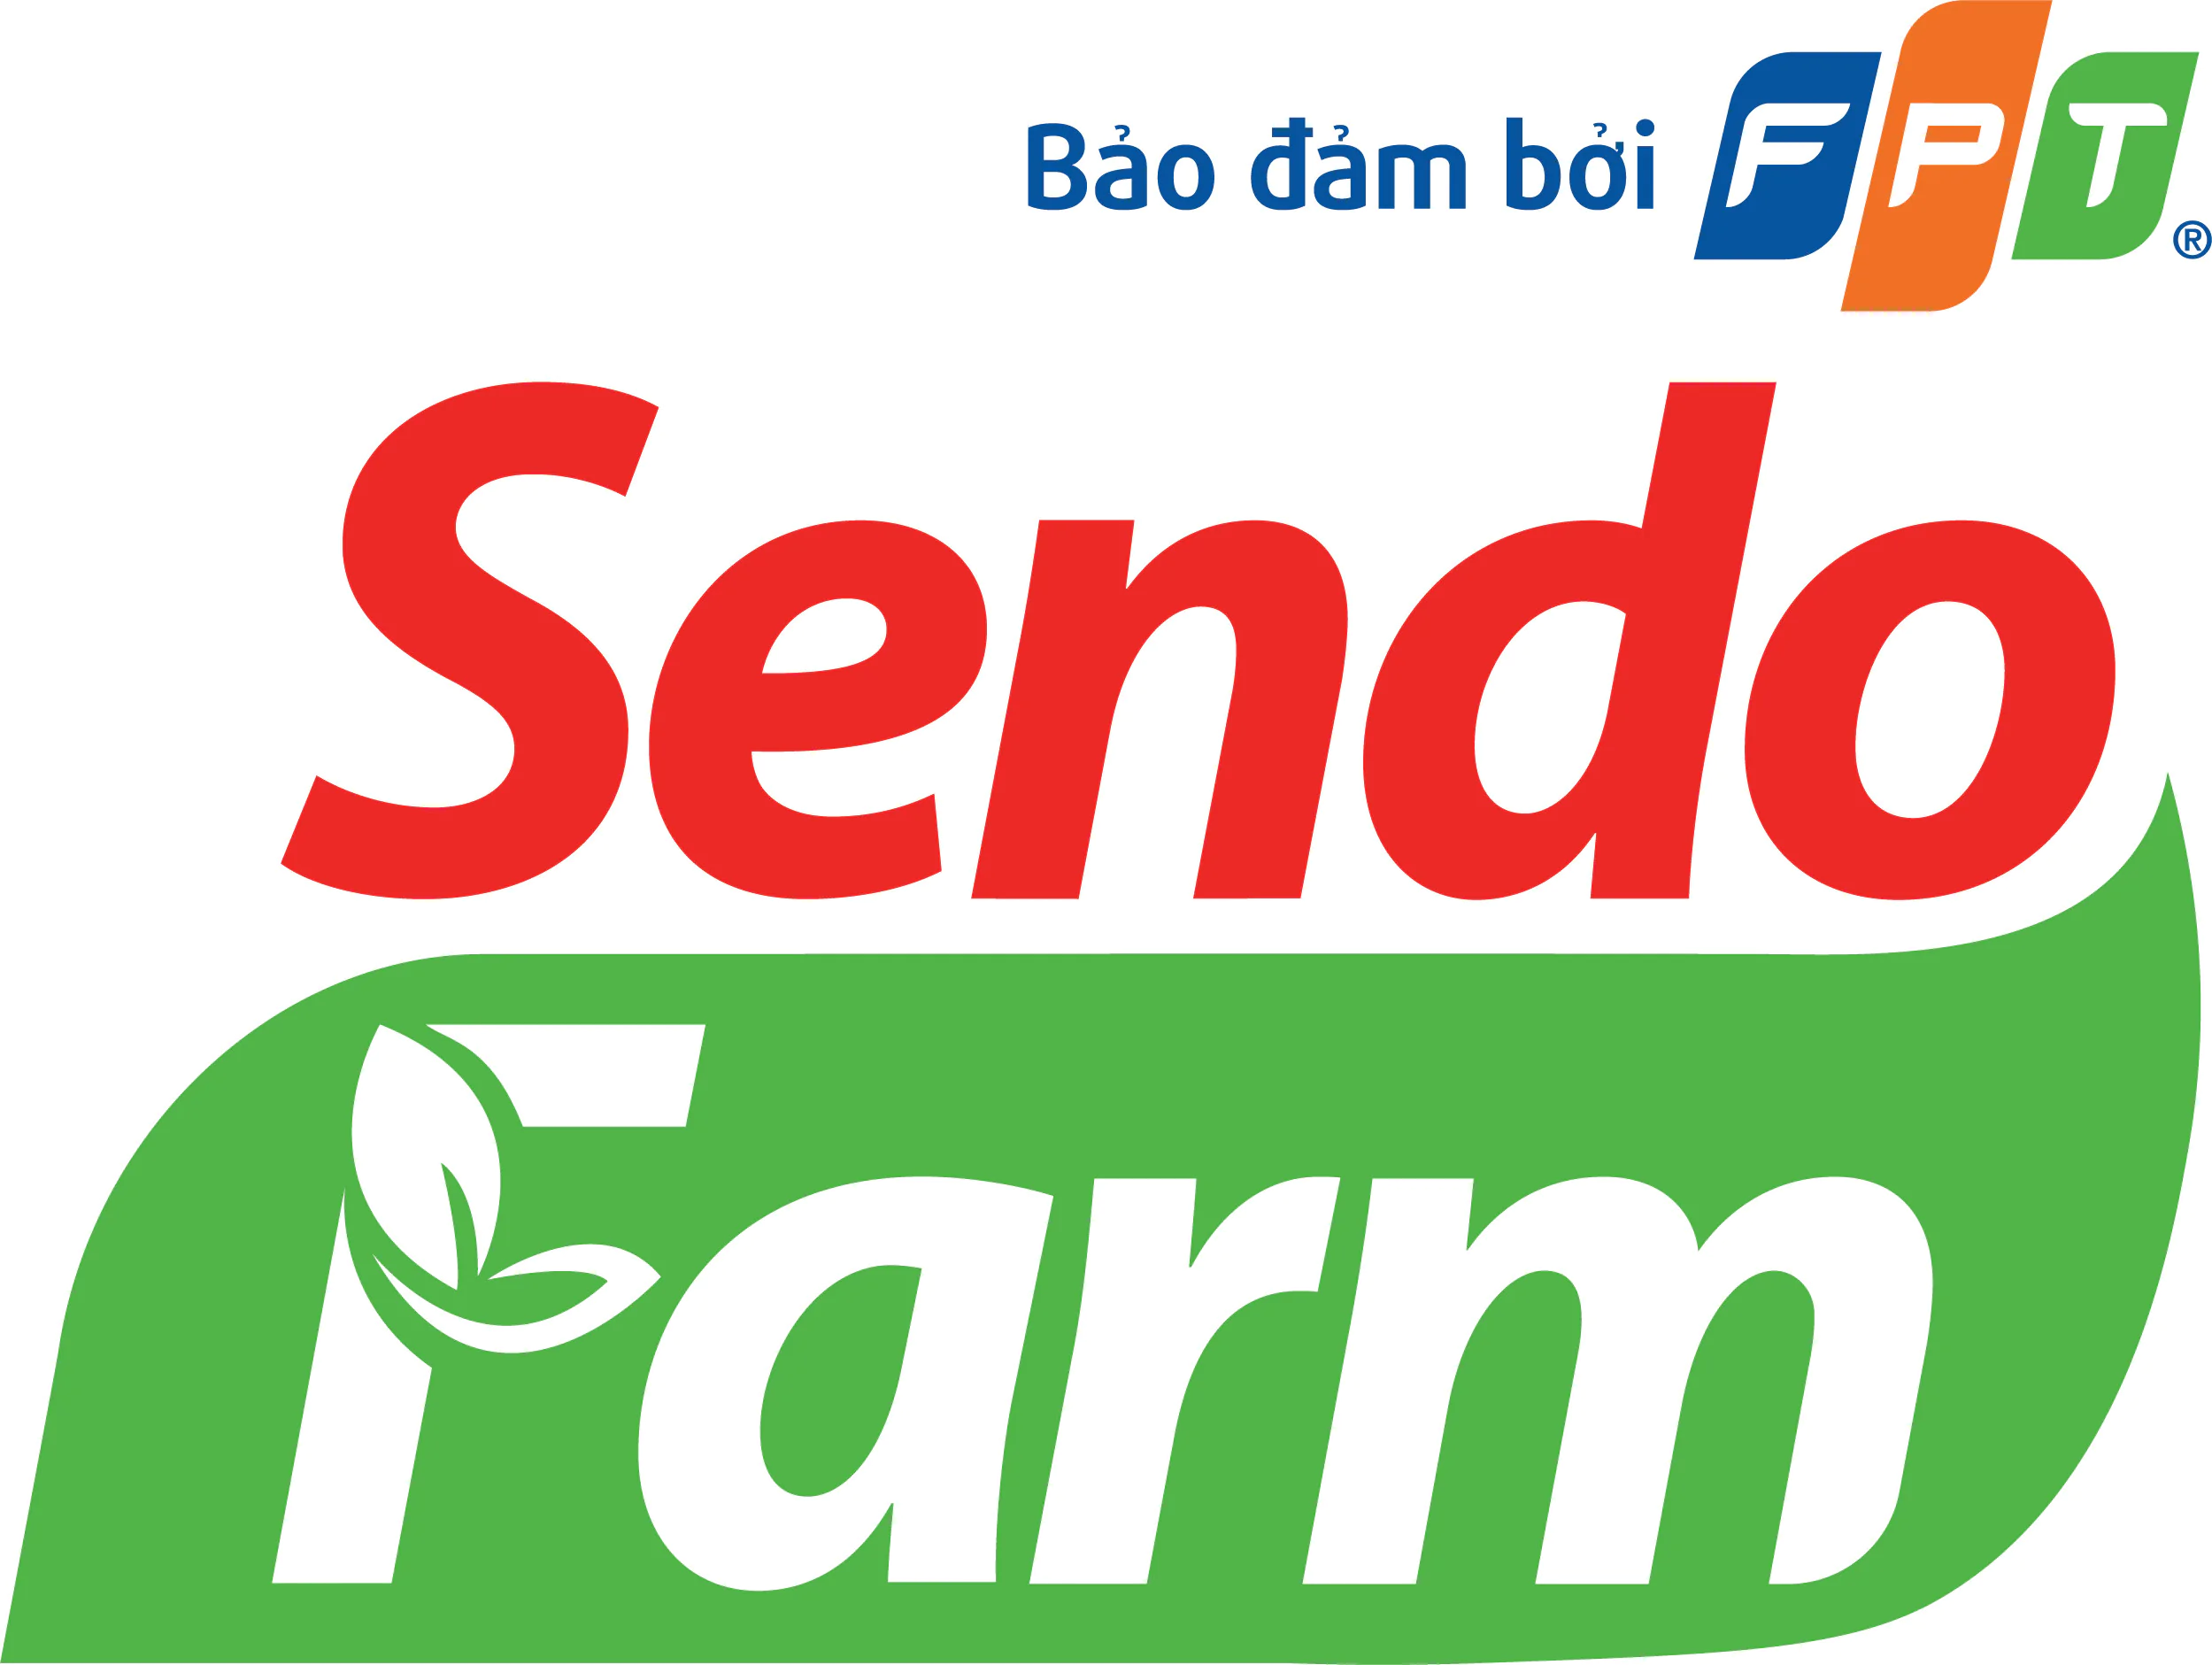
\includegraphics[width=5cm]{Images/sendo.png}
\end{center}
\end{figure}

\begin{itemize}
    \item \textbf{Điểm mạnh:}
        \begin{itemize}
            \item Với lợi thế có sẵn từ Sendo, giúp Sendo Farm có sẵn một lượng lớn người tiêu dùng.
            \item Chuyển đổi từ Sendo thường sang Sendo Farm rất dễ dàng, việc tích hợp chung với Sendo thường giúp tận dụng được lượng khách hàng có sẵn từ Sendo.
            \item Chất lượng đảm bảo bởi FPT - một tập đoàn uy tín ở Việt Nam.
            \item Đã hợp tác xã với rất nhiều địa phương để thúc đẩy tình hình kinh tế ở các địa phương đó, điều này cũng góp phần làm tăng độ uy tín của ứng dụng.
            \item Liên kết với rất nhiều ví điện tử và ngân hàng, giúp việc thanh toán online dễ dàng.
            \item Cách thức vận hành khác biệt so với các sàn thương mại điện tử trên thị trường.
            \item Thời gian nhận hàng nhanh, được cam kết bởi ứng dụng - “Mua hôm nay, mai nhận ngay”.
            \item Nhờ cách thức vận hành đặc biệt nên luôn được miễn phí giao hàng, khách hàng chỉ cần đi quãng đường ngắn là đã mua được nông sản tươi và một số nông sản không có ở gần nơi ở. Nhờ đó thu hút một nhóm khách hàng tiềm năng khác.
            \item Thu hút thêm một lượng lớn người dùng với mục đích đăng ký làm điểm nhận hàng.
            \item Có thể chọn thời gian nhận hàng tùy ý.
        \end{itemize}
    \item \textbf{Điểm yếu:}
        \begin{itemize}
            \item Chỉ có trên nền tảng điện thoại, chưa có website.
            \item Không có phương thức thanh toán trực tiếp.
            \item Thời gian cho phép hủy đơn quá ngắn (5 phút).
            \item Bộ lọc không đa dạng như một số sàn khác trên thị trường.
            \item Điểm nhận hàng chưa có mặt ở những địa phương xa thành phố.
            \item Sản phẩm không đa dạng do bị giới hạn bởi khu vực.
        \end{itemize}
\end{itemize}

\subsection{Kết luận}
\begin{itemize}
    \item \textbf{Tối ưu hóa cho các cửa hàng nhỏ tại Việt Nam:}
        \begin{itemize}
            \item Các hệ thống kể trên hướng đến cả doanh nghiệp nhỏ, vừa và lớn, nên có rất nhiều chức năng phức tạp, có thể khiến người dùng bối rối khi sử dụng. Bên cạnh đó, những gì mà nhiều cửa hàng nhỏ cần thực sự chỉ là một số chức năng nhỏ trong số rất nhiều chức năng mà hệ thống cung cấp. Ví dụ, mục tiêu chính của một số cửa hàng chỉ là bán sản phẩm, in hóa đơn và xem thống kê mà không cần quản lý hàng tồn kho. 
            \item Do đó, hệ thống sẽ kế thừa, cải tiến cũng như đơn giản hóa một số chức năng cơ bản của các hệ thồng trên như các giao dịch mua bán, hoàn trả hàng, quản lý hàng tồn kho, khách hàng, báo cáo và thống kê, sẽ dễ sử dụng hơn, đơn giản hơn và phù hợp với các nhà bán lẻ nhỏ ở Việt Nam.
        \end{itemize}
    \item \textbf{Thêm một số chức năng tự động hóa cơ bản:}
        \begin{itemize}
            \item Hệ thống sẽ hỗ trợ một số chức năng tự động hóa cơ bản giúp người dùng giảm thiểu sai sót trong các công việc thủ công khi quản lý tồn kho như thông báo để cảnh báo sản phẩm sắp hết hàng hoặc sản phẩm sắp hết hạn. Ngoài ra, hệ thống sẽ hỗ trợ một số chức năng giúp quy trình làm việc của cửa hàng hiệu quả hơn.
        \end{itemize}
    \item \textbf{Giao diện người dùng thân thiện hơn:}
        \begin{itemize}
            \item Một trong những yếu tố quan trọng ảnh hưởng đến quyết định của người dùng xem họ sẽ sử dụng hệ thống hay không, không chỉ là các tính năng cần thiết, tính bảo mật, hiệu suất, mà còn là giao diện người dùng. Vì giao diện người dùng là yếu tố đầu tiên thu hút người dùng quyết định sử dụng một hệ thống. Nhiều người dùng cần một giao diện thân thiện về cả thiết kế giao diện người dùng và trải nghiệm người dùng. Nên việc tập trung xây dựng một giao diện thân thiện với người dùng là một yếu tố quan trọng quyết định khả năng thành công cảu hệ thống.
        \end{itemize}
\end{itemize}